\chapter{Prakter Apex Oracle}

\section{Langkah Kerja}
\begin{enumerate}
 \item Pertama,olah data yang didapat. Pengolahan data dibutuhkan agar data yang dimasukkan kedalam database tidak terdapat kesalahan dan redudansi.
  \begin{figure}[H]
    \centering
    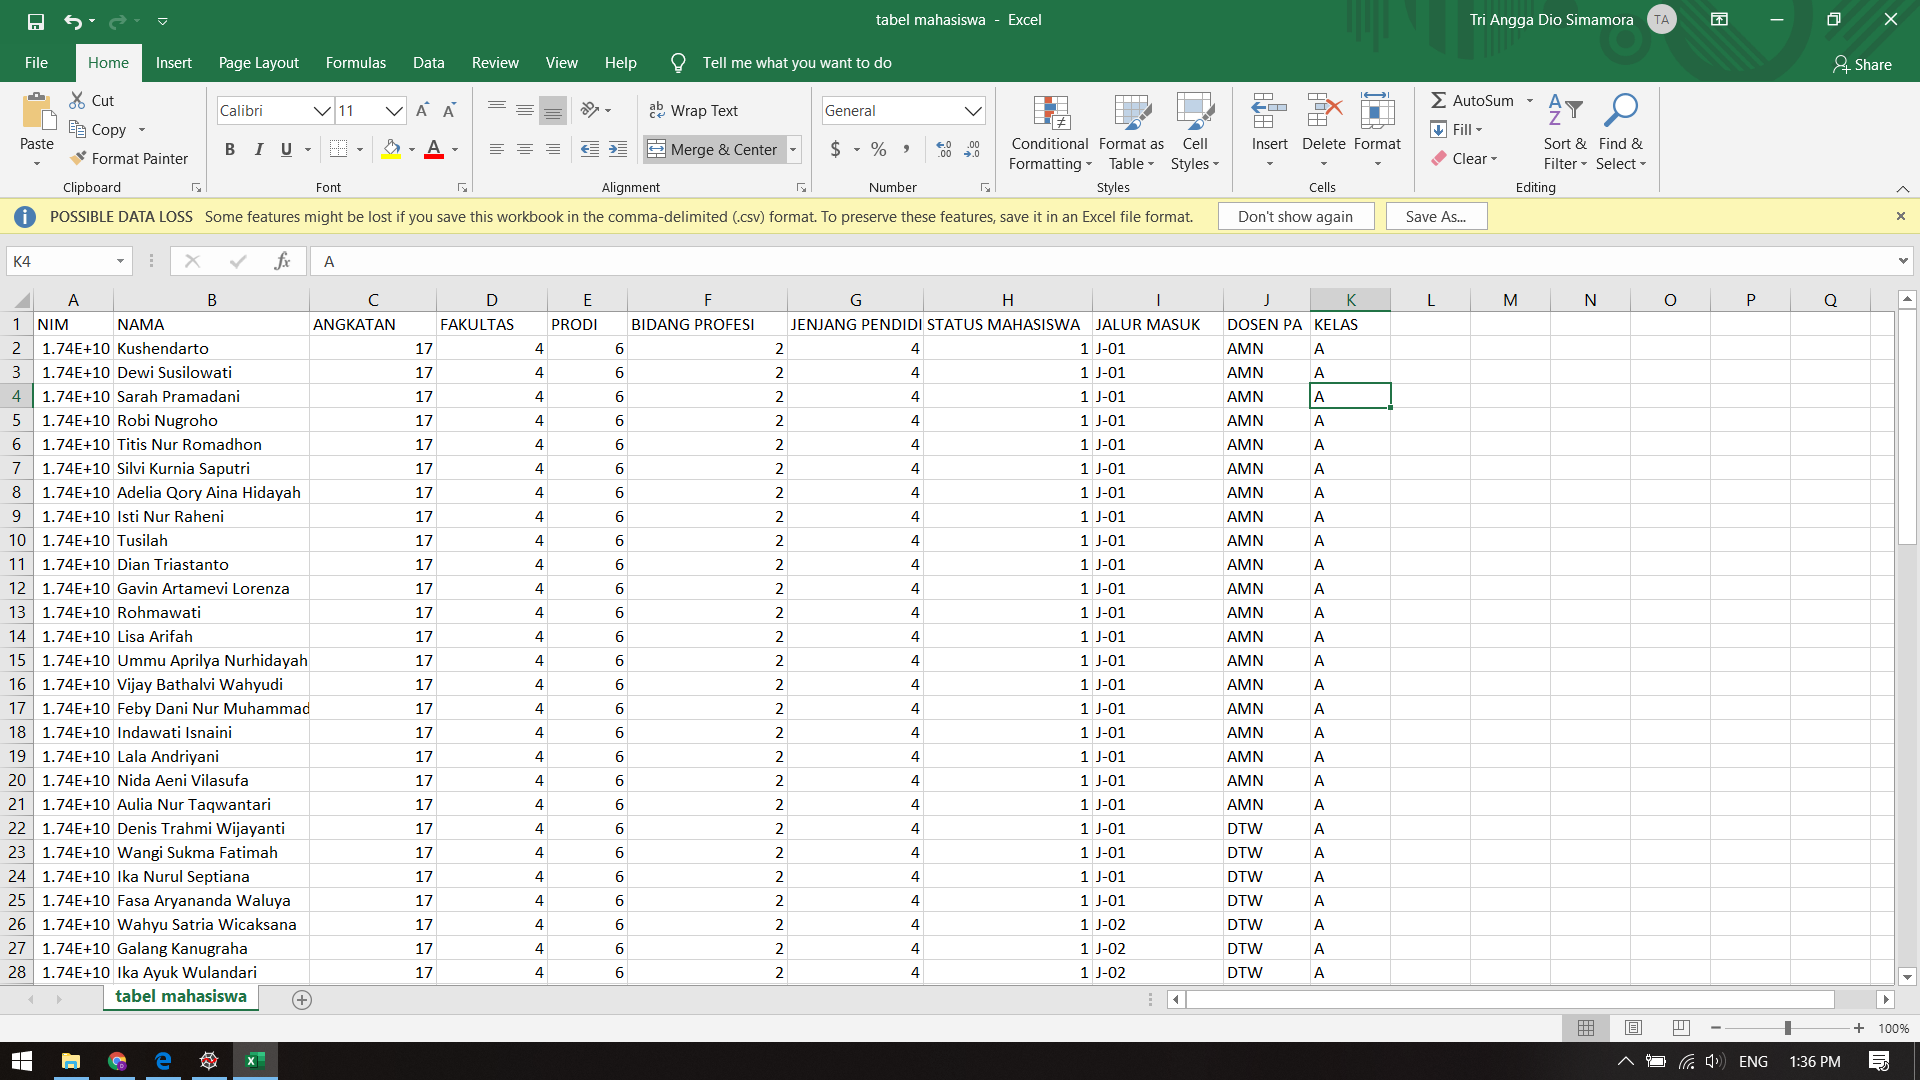
\includegraphics[scale=0.3]{figures/data mentah}
    \caption{\textit{Data yang Diolah}}
    \label{foto11}
 \end{figure}
 \item Pisahkan data menjadi beberapa tabel data.
 \item Berikan kode pada masing-masing data yang nanti akan berperan sebagai primary key.
 \item Buka Apex oracle online. Click App Builder, kemudian klik create, pilih from a file.
 \begin{figure}[H]
    \centering
    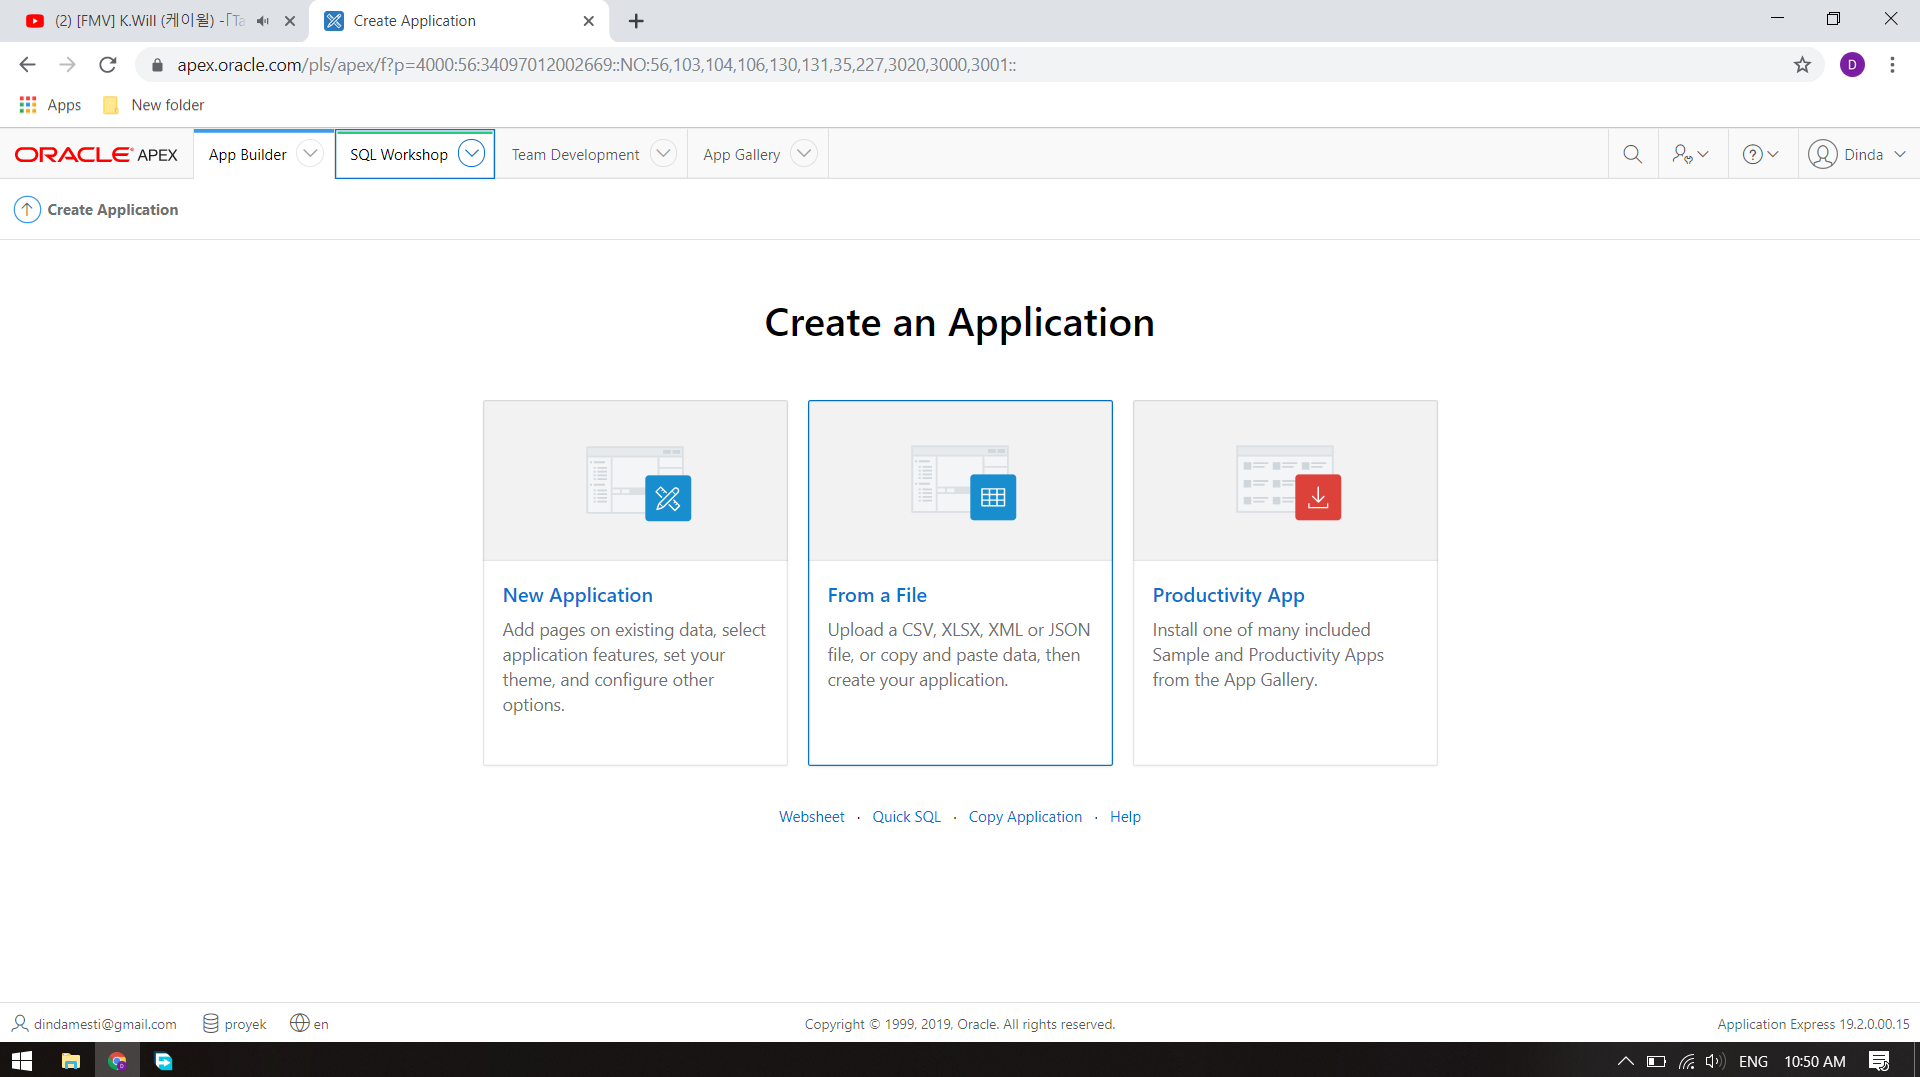
\includegraphics[scale=0.3]{figures/4}
    \caption{\textit{From a File}}
    \label{foto3}
 \end{figure}
 \item Pilih choose file, kemudian pilih file csv yang akan di load. Load semua table yang telah kita buat satu per satu.
 \begin{figure}[H]
    \centering
    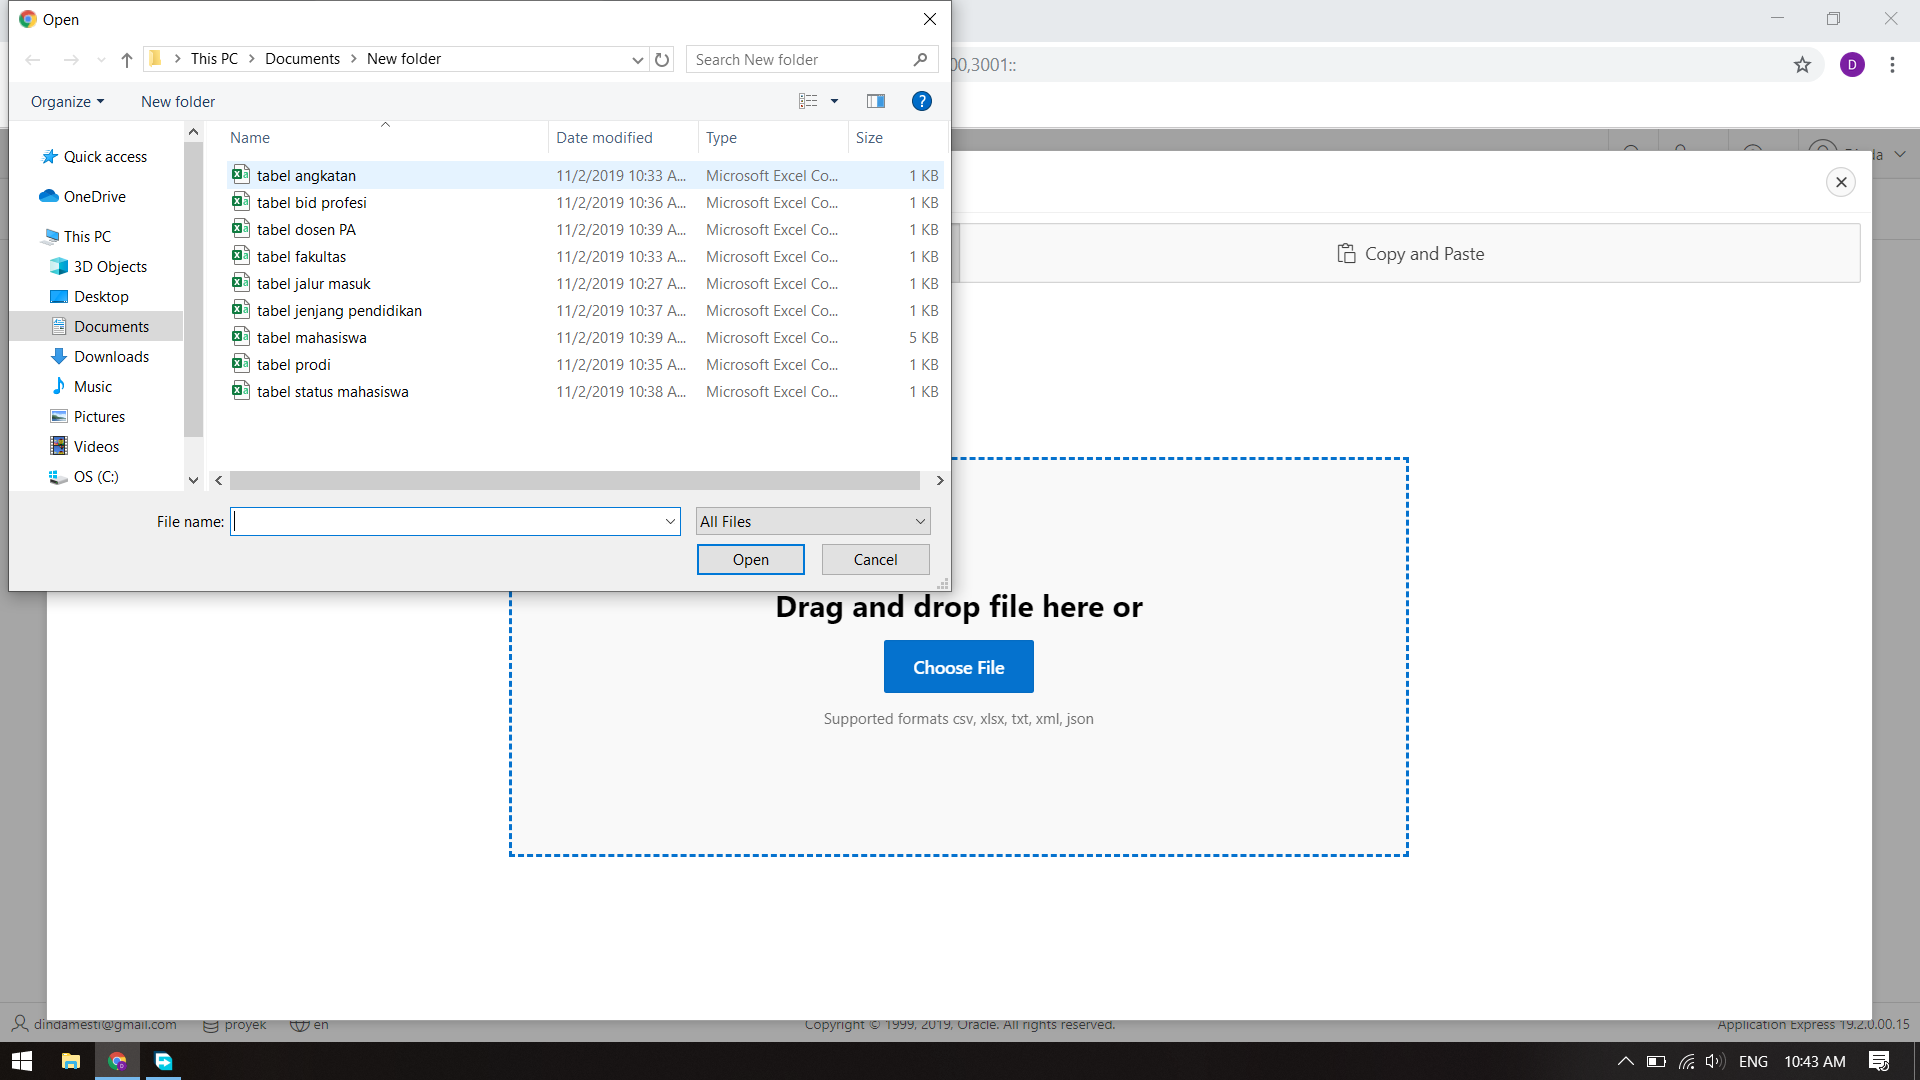
\includegraphics[scale=0.3]{figures/1}
    \caption{\textit{Pilih File CSV}}
    \label{foto1}
 \end{figure}
 \item Ketika diminta untuk mengisikan nama tabel, maka isikan nama tabel dan pastikan data didalam tabel telah diload dengan sempurna dengan cara mengklik configure.
 \begin{figure}[H]
    \centering
    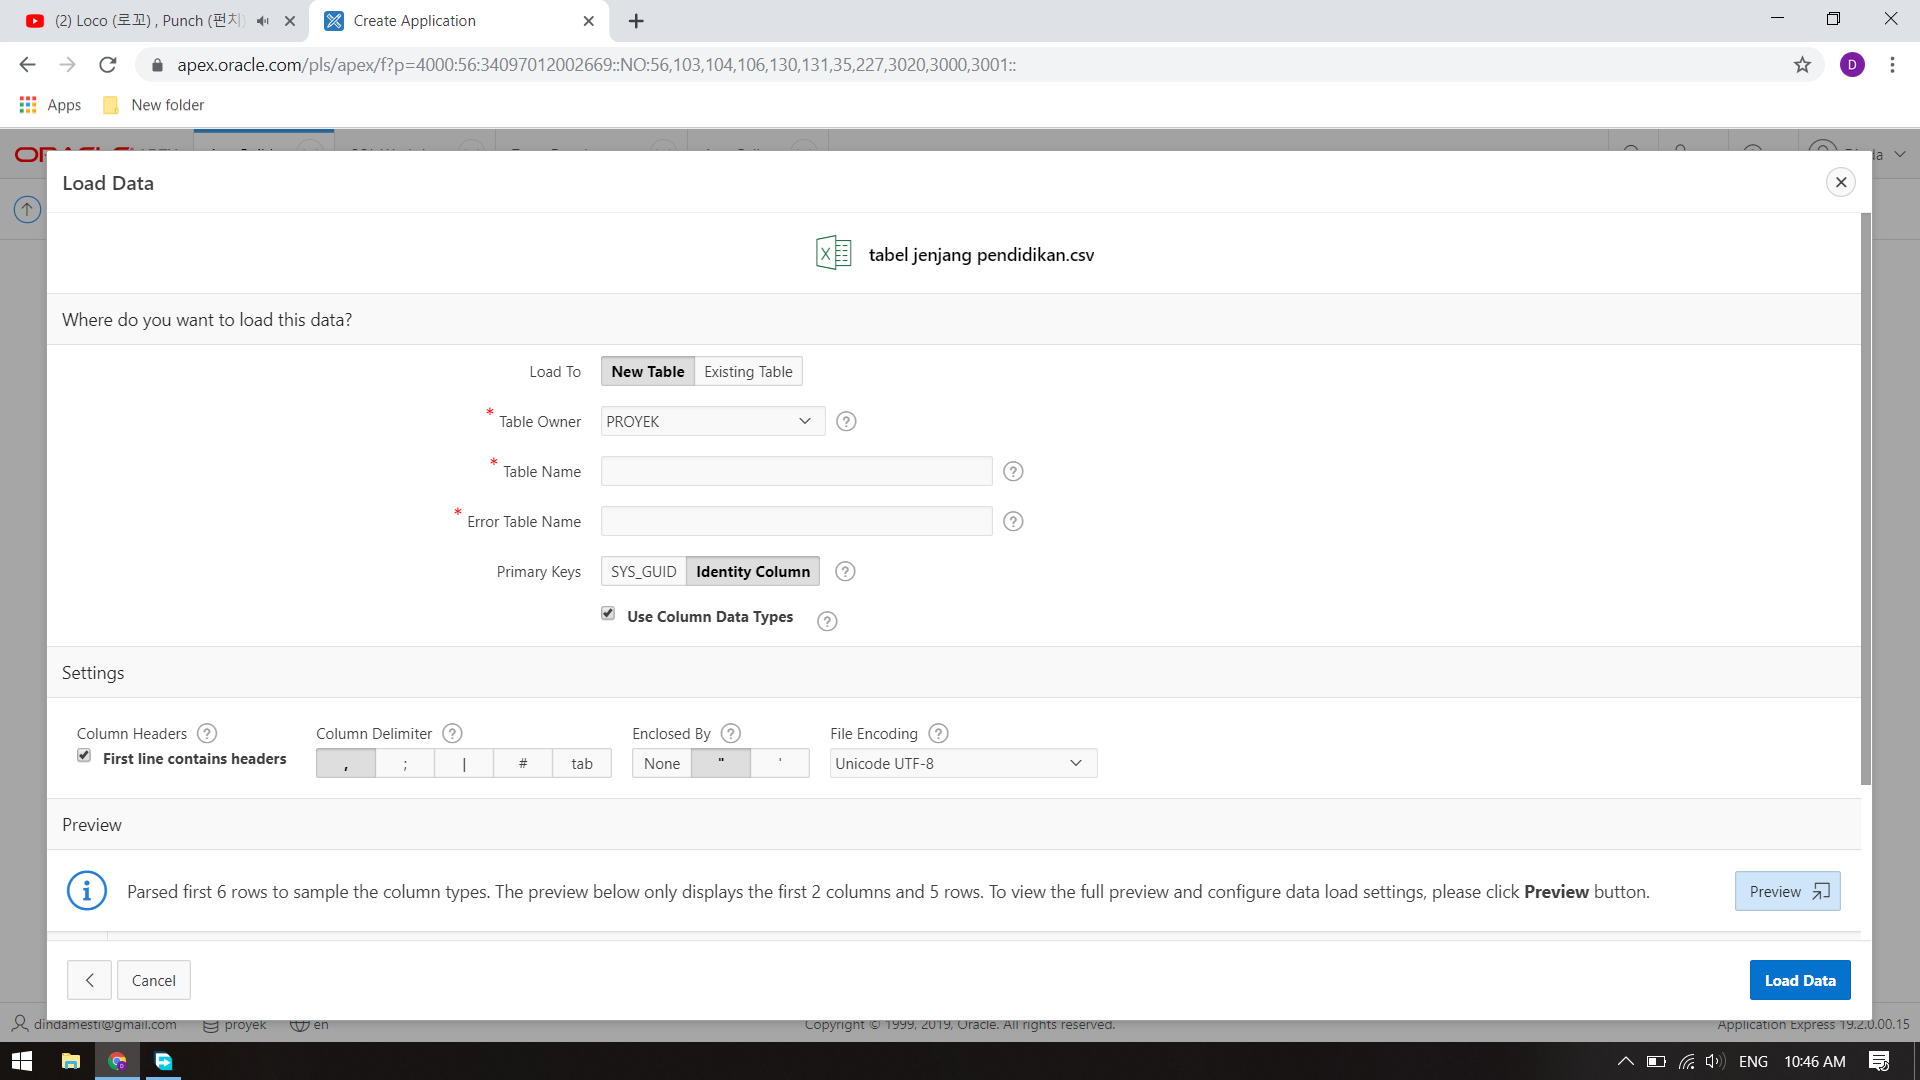
\includegraphics[scale=0.3]{figures/2}
    \caption{\textit{Form Nama Tabel}}
    \label{foto2}
 \end{figure}
 \item Apabila semua file tabel telah di load, maka tabel tersebut akan muncul di Object Browser. Kemudian edit semua tabel yang telah diload dengan melakukan drop column, kemudian pilih column ID sebagai column yang akan dihapus.
 \begin{figure}[H]
    \centering
    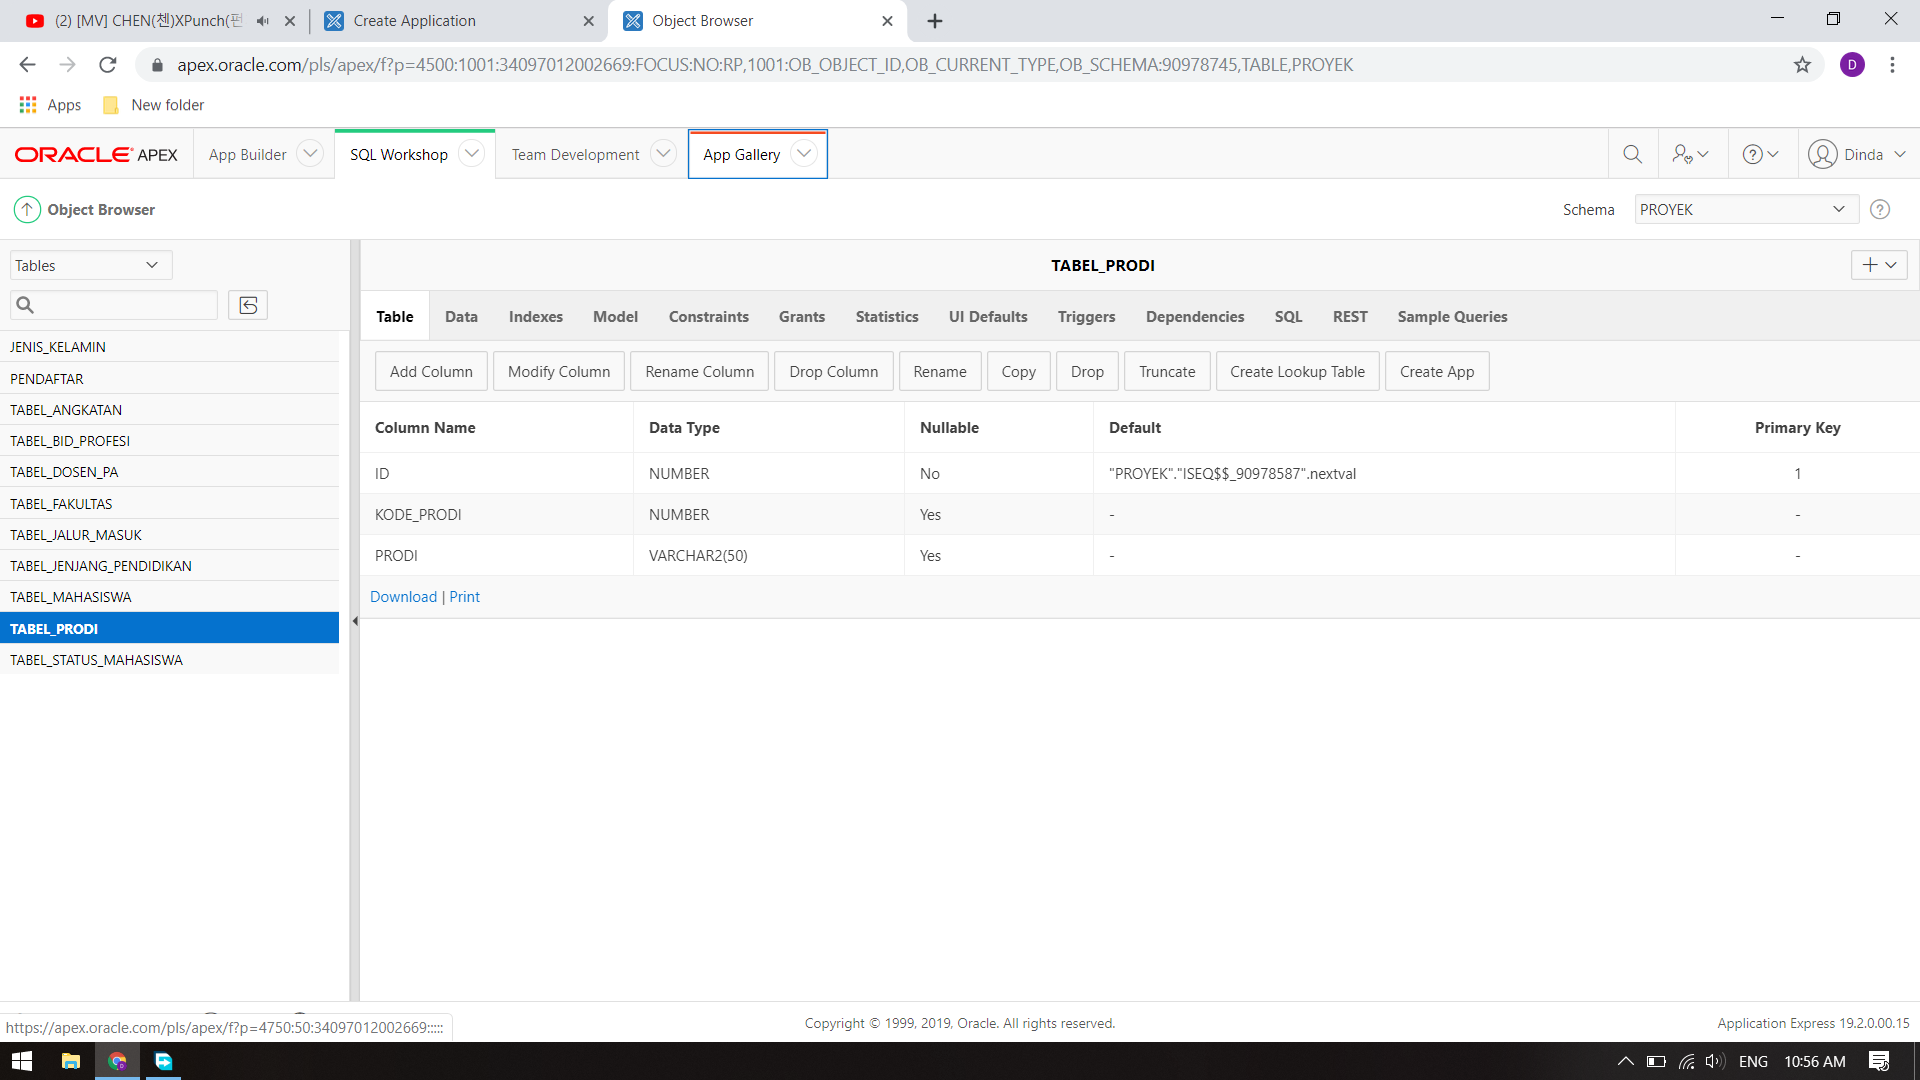
\includegraphics[scale=0.3]{figures/7}
    \caption{\textit{Object Browser}}
    \label{foto4}
 \end{figure}
 \item Buka SQL Command, Ketikkan perintah SQL untuk menambahkan primary key pada setiap tabel yang telah di load dan dihapus ID nya. Kemudian ketikkan perintah SQL untuk menambahkan foreign key dari satu tabel ke tabel lainnya. Pastikan untuk menjalankan perintah SQL diblock terlebih dahulu baris kode yang akan dijalankan.
 \begin{verbatim}
ALTER TABLE TABEL_ANGKATAN
ADD PRIMARY KEY (KODE_ANGKATAN);

ALTER TABLE TABEL_MAHASISWA
ADD FOREIGN KEY (KODE_ANGKATAN) 
REFERENCES TABEL_ANGKATAN (KODE_ANGKATAN);

ALTER TABLE TABEL_FAKULTAS
ADD PRIMARY KEY (KODE_FAKULTAS);

ALTER TABLE TABEL_MAHASISWA
ADD FOREIGN KEY (KODE_FAKULTAS) 
REFERENCES TABEL_FAKULTAS (KODE_FAKULTAS);

ALTER TABLE TABEL_PRODI
ADD PRIMARY KEY (KODE_PRODI);

ALTER TABLE TABEL_MAHASISWA
ADD FOREIGN KEY (KODE_PRODI) 
REFERENCES TABEL_PRODI (KODE_PRODI);

ALTER TABLE TABEL_BID_PROFESI
ADD PRIMARY KEY (KODE_BID_PROFESI);

ALTER TABLE TABEL_MAHASISWA
ADD FOREIGN KEY (KODE_BID_PROFESI) 
REFERENCES TABEL_BID_PROFESI (KODE_BID_PROFESI);

ALTER TABLE TABEL_JENJANG_PENDIDIKAN
ADD PRIMARY KEY (KODE_JENJANG);

ALTER TABLE TABEL_MAHASISWA
ADD FOREIGN KEY (KODE_JENJANG) 
REFERENCES TABEL_JENJANG_PENDIDIKAN (KODE_JENJANG);

ALTER TABLE TABEL_STATUS_MAHASISWA
ADD PRIMARY KEY (KODE_STATUS_MAHASISWA);

ALTER TABLE TABEL_MAHASISWA
ADD FOREIGN KEY (KODE_STATUS_MAHASISWA) 
REFERENCES TABEL_STATUS_MAHASISWA (KODE_STATUS_MAHASISWA);

ALTER TABLE TABEL_JALUR_MASUK
ADD PRIMARY KEY (KODE_JALUR_MASUK);

ALTER TABLE TABEL_MAHASISWA
ADD FOREIGN KEY (KODE_JALUR_MASUK) 
REFERENCES TABEL_JALUR_MASUK (KODE_JALUR_MASUK);

ALTER TABLE TABEL_DOSEN_PA
ADD PRIMARY KEY (KODE_DOSEN_PA);

ALTER TABLE TABEL_MAHASISWA
ADD FOREIGN KEY (KODE_DOSEN_PA) 
REFERENCES TABEL_DOSEN_PA (KODE_DOSEN_PA);
 \end{verbatim}
 \begin{figure}[H]
    \centering
    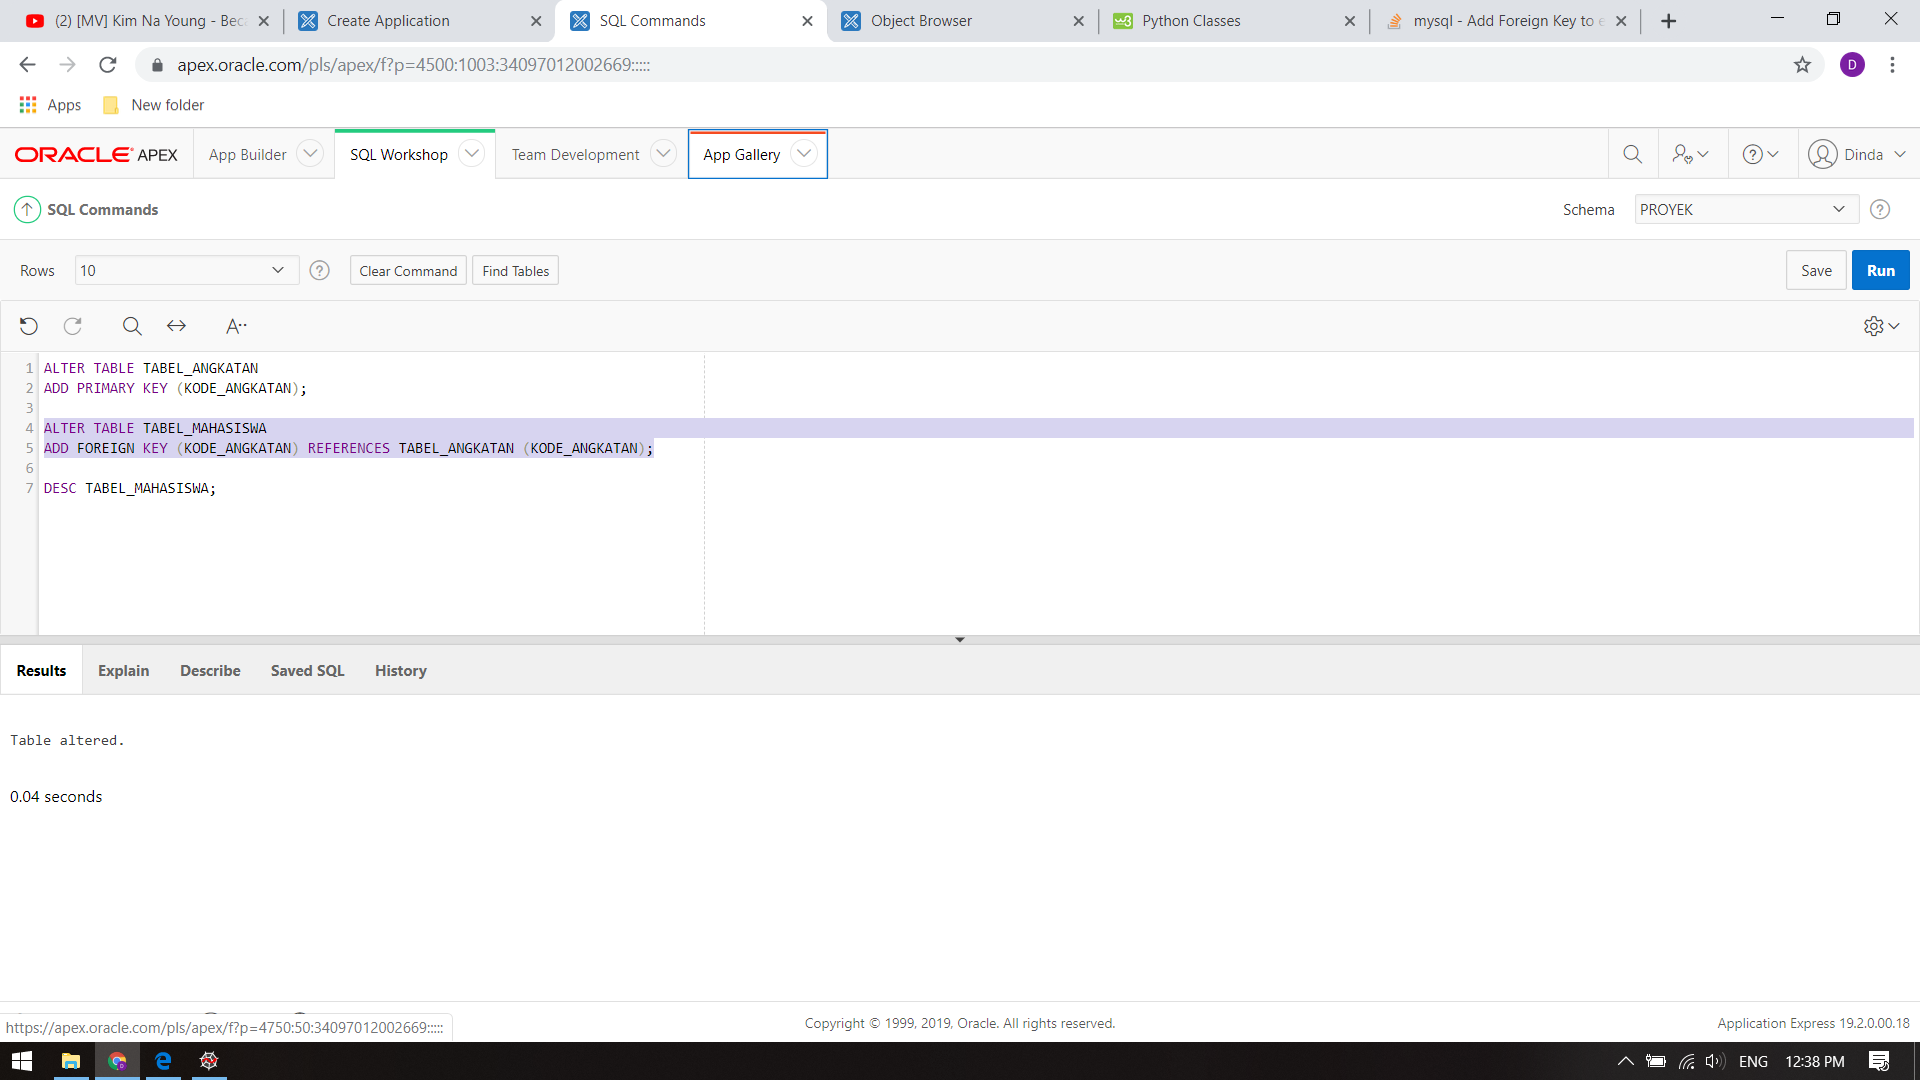
\includegraphics[scale=0.3]{figures/8}
    \caption{\textit{Run Command}}
    \label{foto5}
 \end{figure}
 \item Cek apakah semua tabel telah memiliki primary key. Bisa dengan menggunakan perintah SQL dan bisa dengan membuka Object Browser dan melihat tabelnya satu per satu. Berikut perintah SQL nya.
 \begin{verbatim}
DESC TABEL_MAHASISWA;
DESC TABEL_ANGKATAN;
DESC TABEL_FAKULTAS;
DESC TABEL_PRODI;
DESC TABEL_BID_PRODESI;
DESC TABEL_JENJANG_PENDIDIKAN;
DESC TABEL_STATUS_MAHASISWA;
DESC TABEL_JALUR_MASUK;
DESC TABEL_DOSEN_PA;
 \end{verbatim}
 \begin{figure}[H]
    \centering
    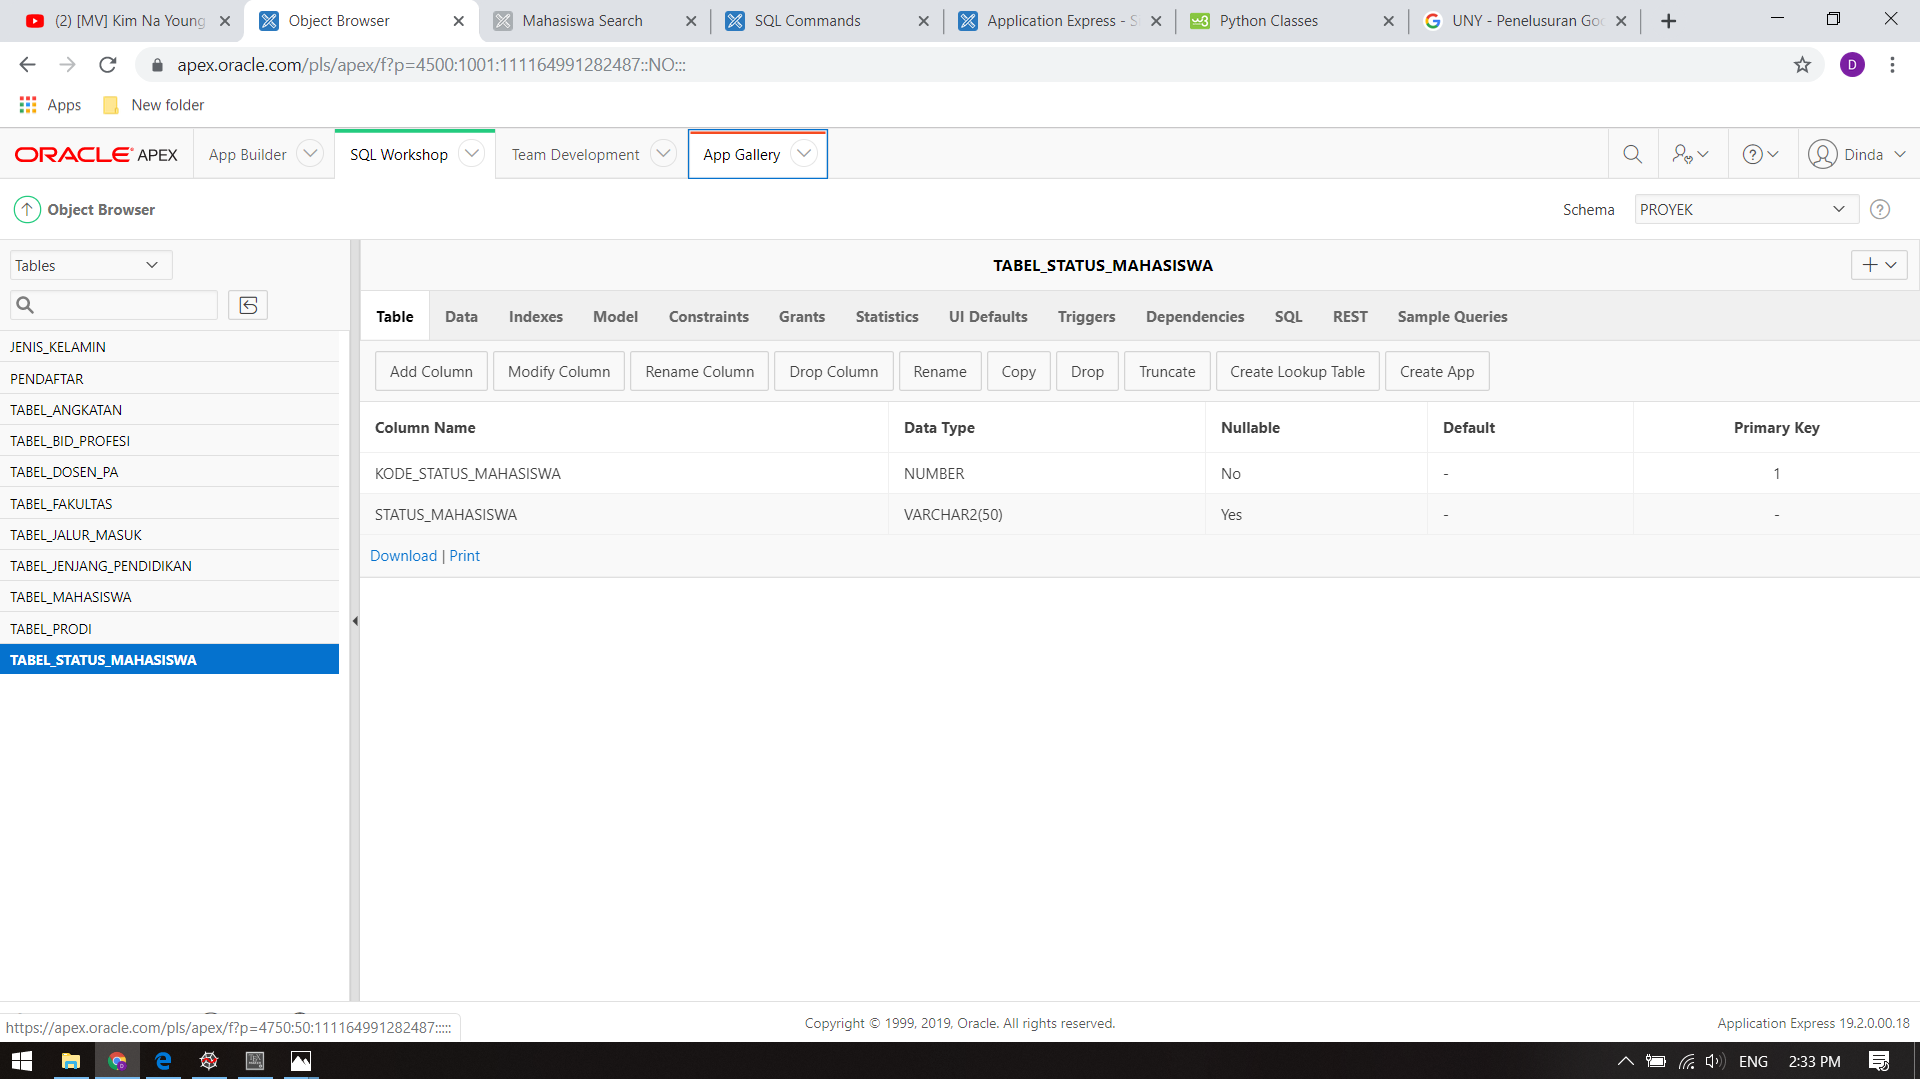
\includegraphics[scale=0.3]{figures/14}
    \caption{\textit{Object Browser Primary}}
    \label{foto6}
 \end{figure}
 \item Jika data sudah selesai dimodifikasi sesuai primary key dan foreign keynya, maka selanjutnya kita buat aplikasinya. Klik App Build, klik create, pilih New Application.
 \begin{figure}[H]
    \centering
    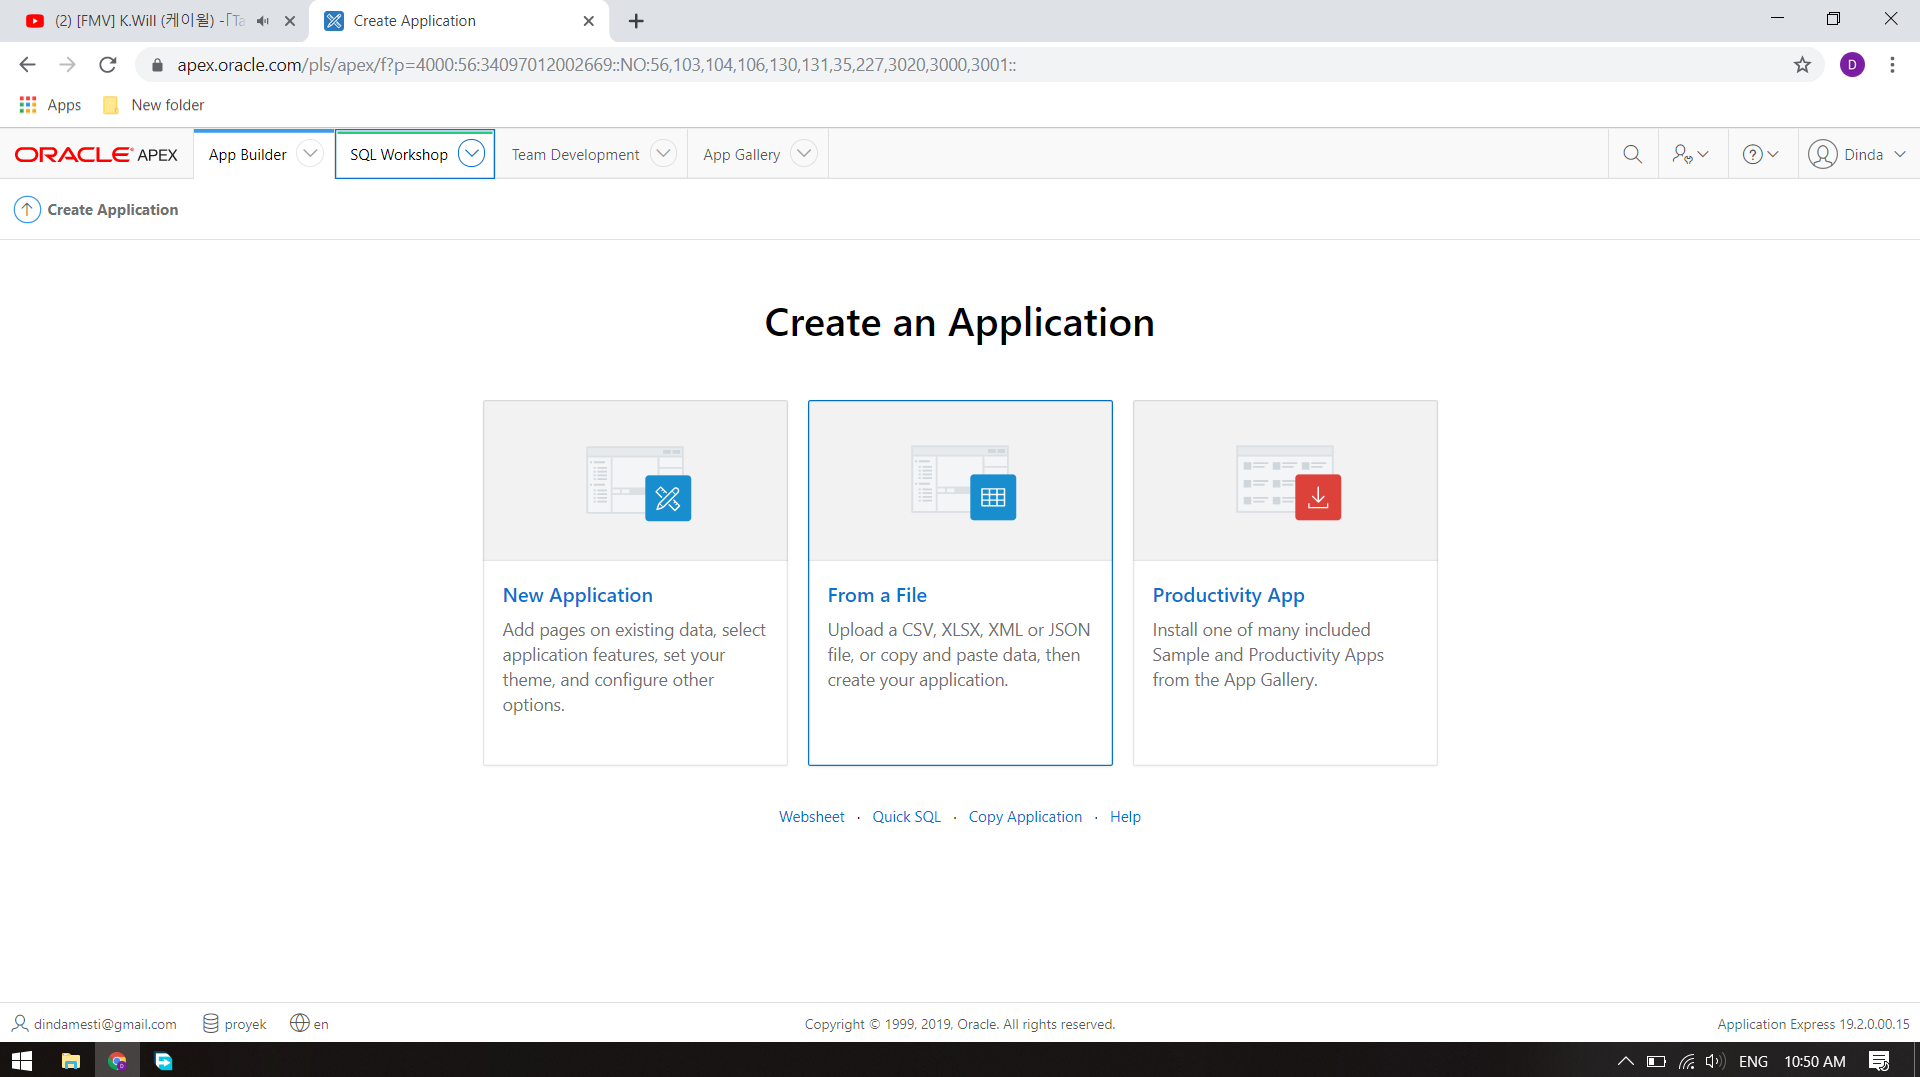
\includegraphics[scale=0.3]{figures/4}
    \caption{\textit{New Application}}
    \label{foto7}
 \end{figure}
 \item Tambahkan page sesuai dengan jumlah tabel yang telah di load.
 \begin{figure}[H]
    \centering
    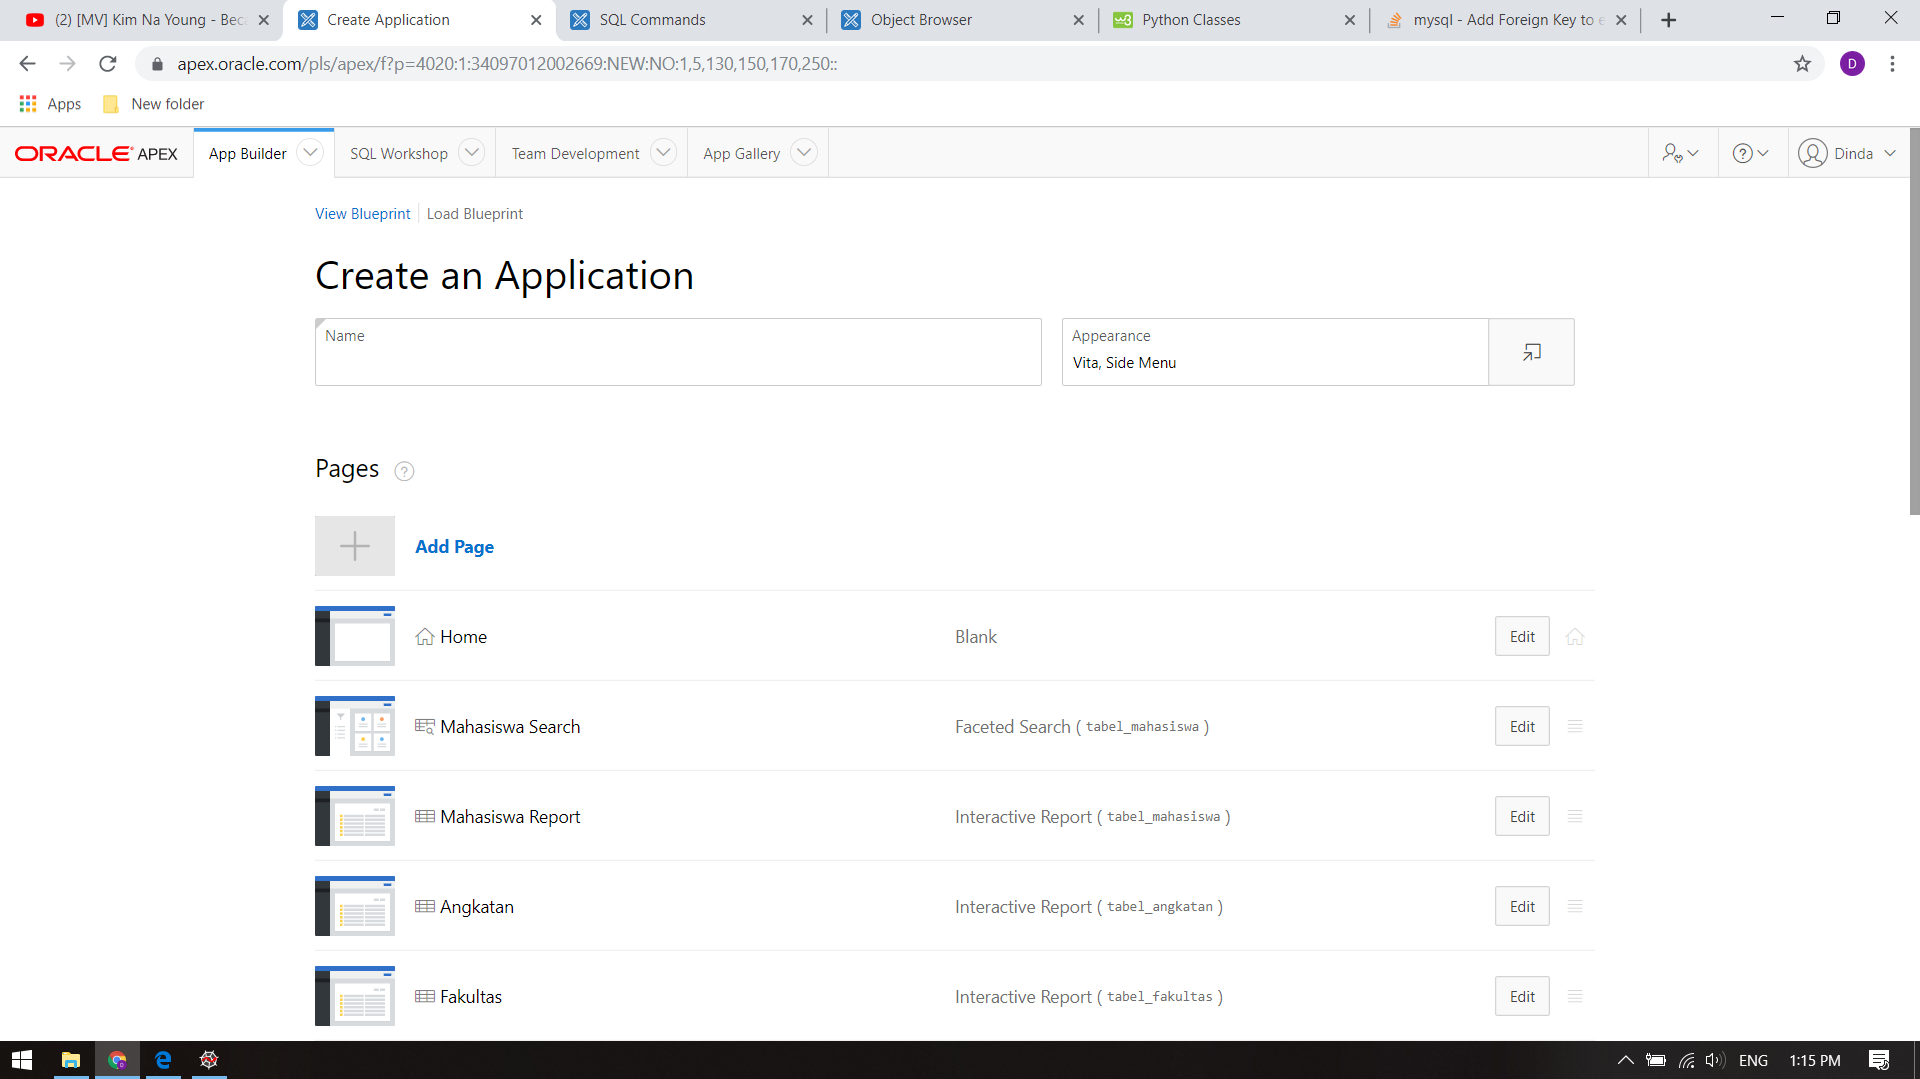
\includegraphics[scale=0.3]{figures/10}
    \caption{\textit{Add Page}}
    \label{foto8}
 \end{figure}
 \item klik create application, kemudian run application, maka akan tampil aplikasi yang telah jadi dan bisa digunakan. Berikut tampilan Home dari aplikasi.
 \begin{figure}[H]
    \centering
    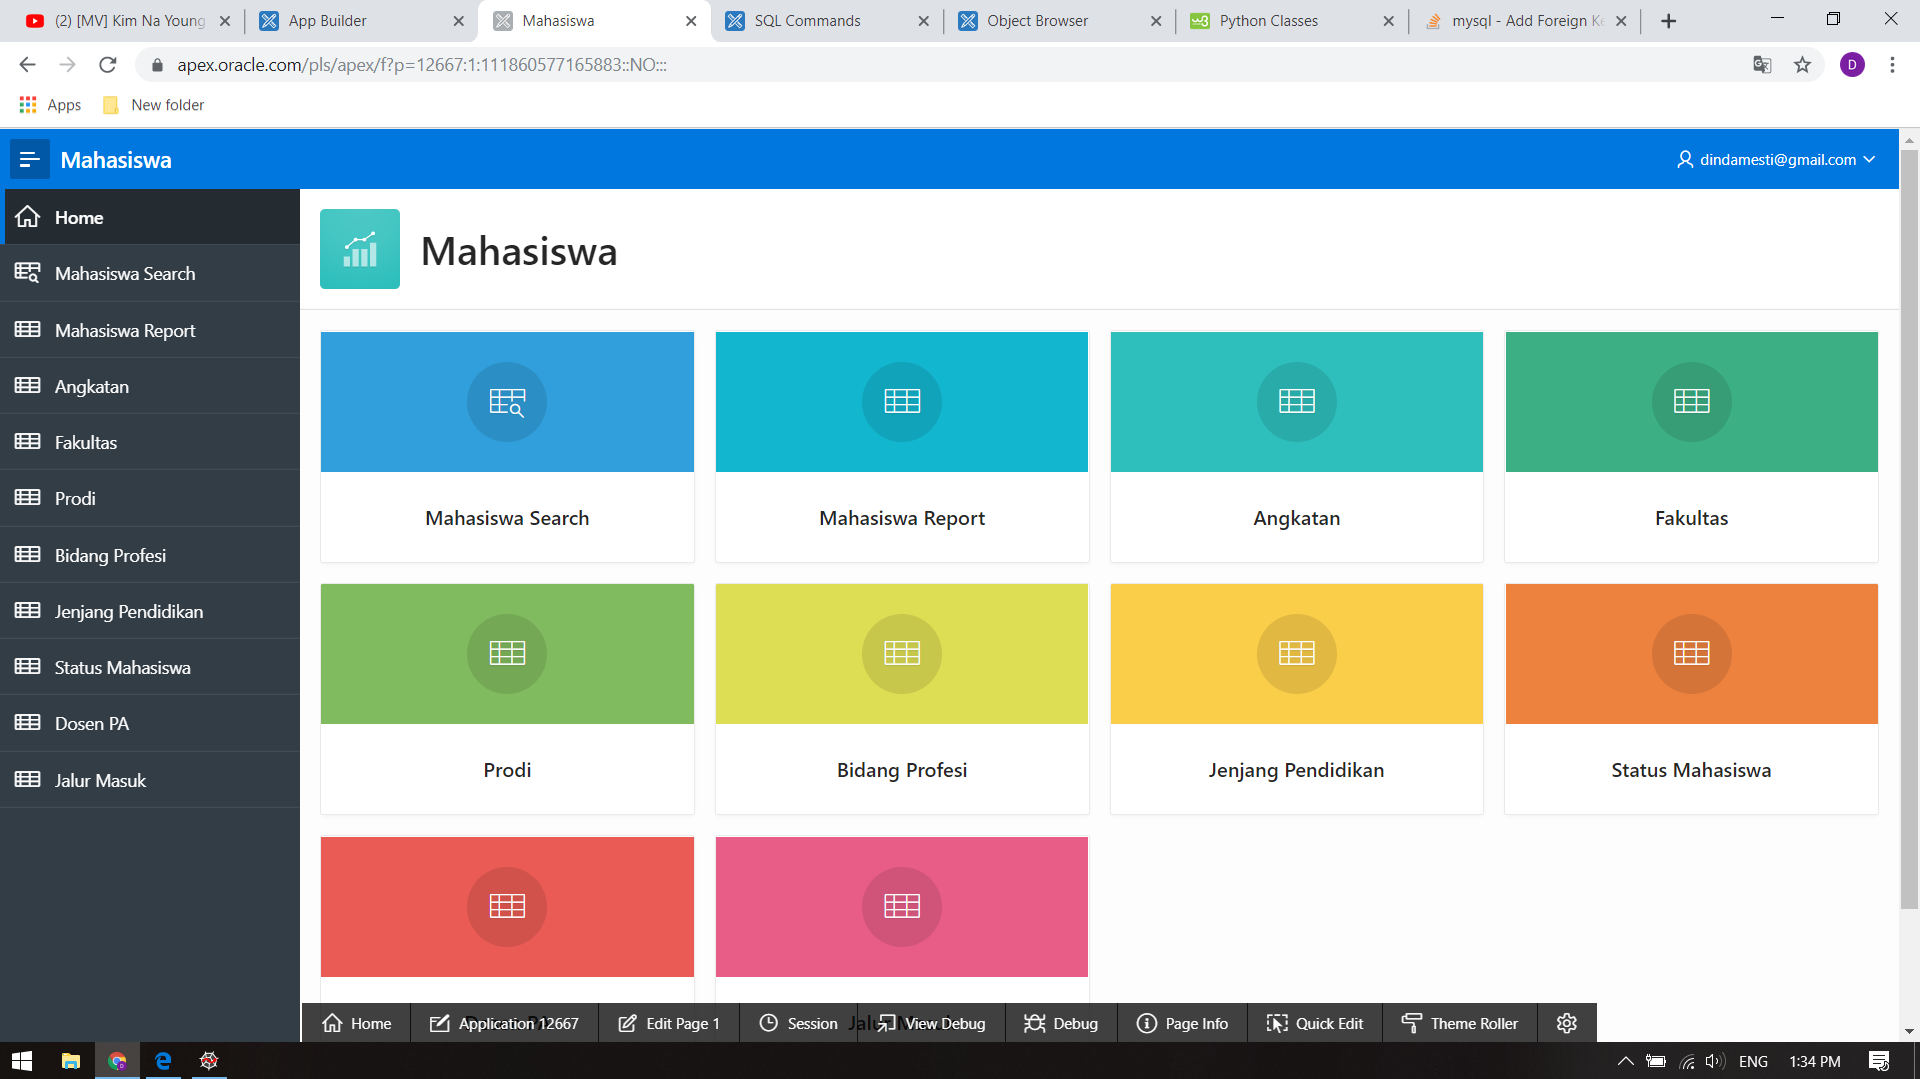
\includegraphics[scale=0.3]{figures/13}
    \caption{\textit{Home Page}}
    \label{foto8}
 \end{figure}
 \item Berikut tampilan Mahasiswa Search
 \begin{figure}[H]
    \centering
    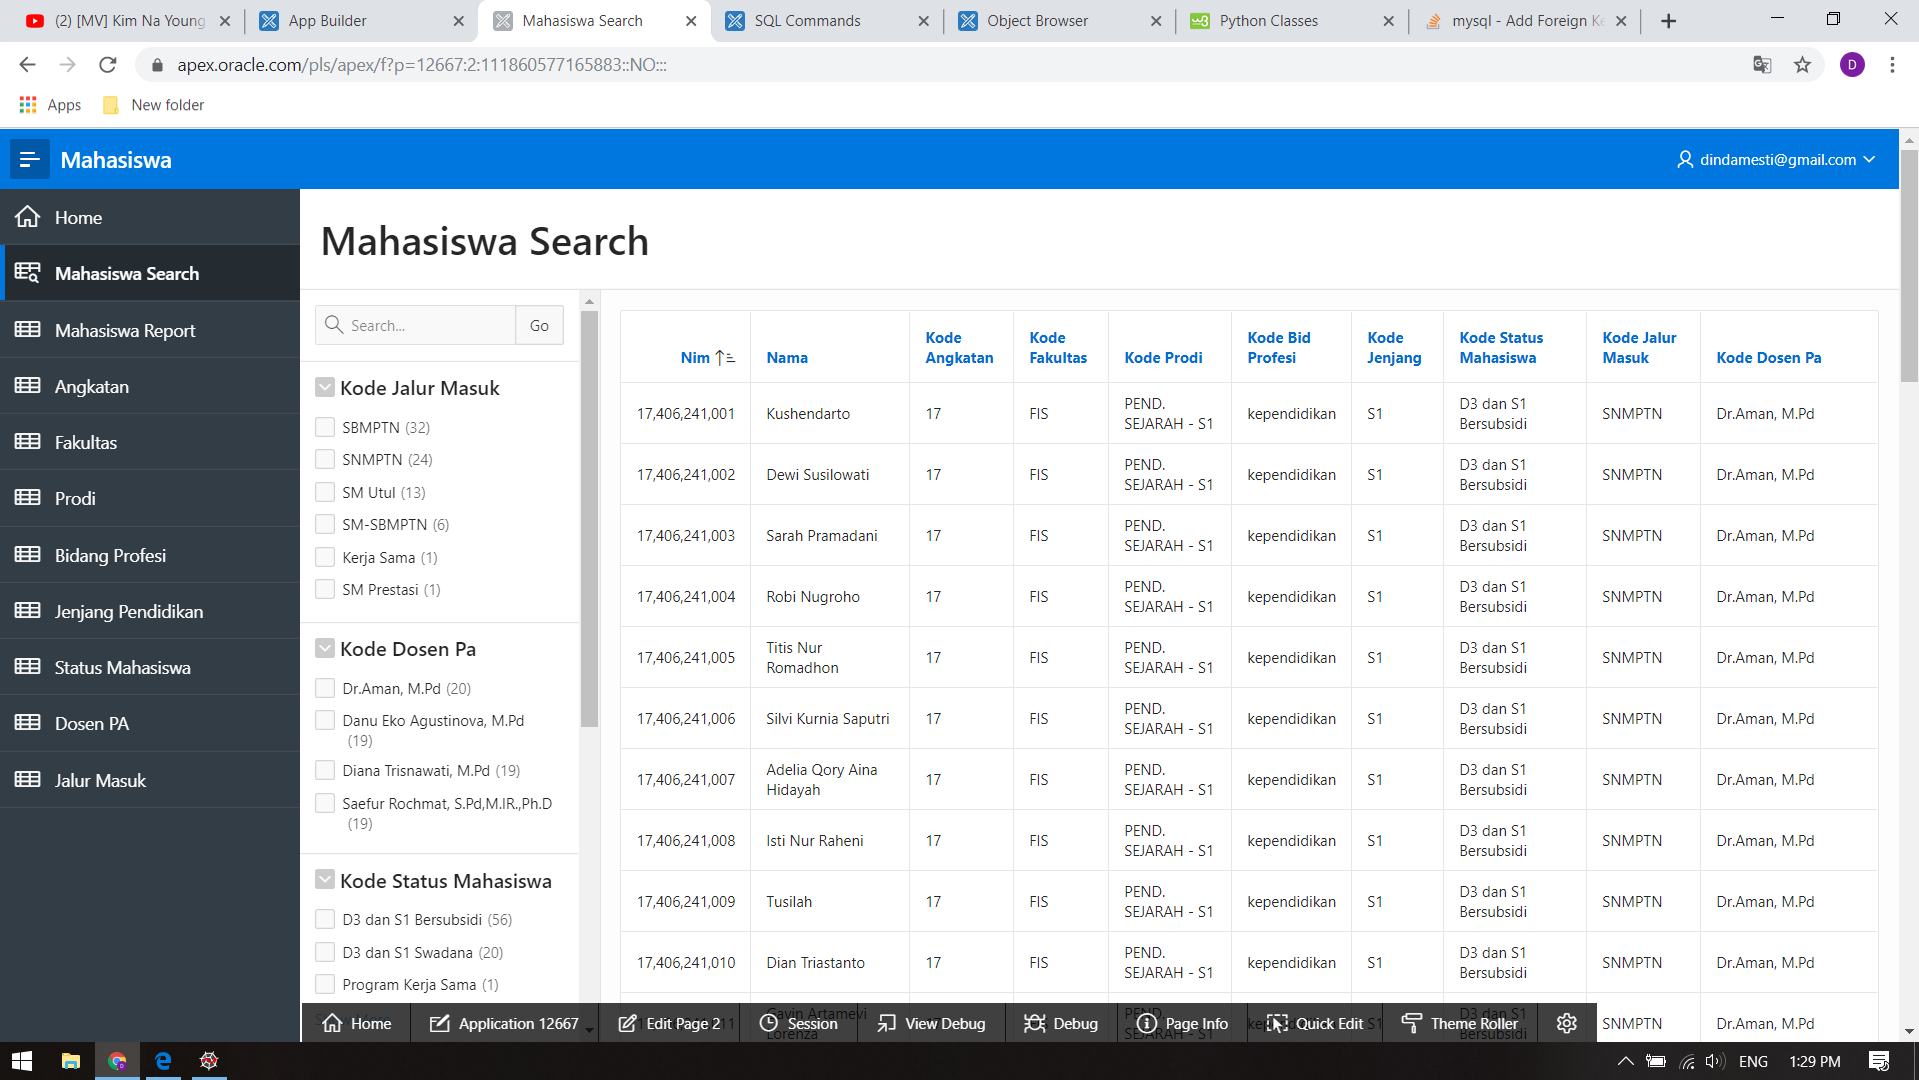
\includegraphics[scale=0.3]{figures/app}
    \caption{\textit{Mahasiswa Search Page}}
    \label{foto8}
 \end{figure}
\end{enumerate}

\subsection{Link Application}
\url{https://apex.oracle.com/pls/apex/f?p=12667:1:31384248786030:::::}\\
Username : dindamesti@gmail.com\\
Password : Dinda130500

